\section{Architecture de la solution}

L'AIPRAO dispose de 3 site à interconnecter:
\begin{description}
\item Le {\bf site central},
\item Le {\bf site GE},
\item Le {\bf site de Roanne}.
\end{description}

\subsection{Interconnexion}

Les sites du réseau de la Doua sont interconnectés via le réseau de campus
ROCAD géré par les DSI des établissements du campus et le CISR.

L'interconnexion avec le site de Roanne est réalisée via le réseau du campus
géré par la DSI de l'université de St Étienne.

Chacun des réseaux de campus est relié à RENATER. 

Les différents sites communiqueront grâce à un VPN.

Les automates programmables, pour ne pas polluer le réseau avec leur
broadcast, seront isolés dans un VLAN. La configuration de ce VLAN
se fait en utilisant le système de {\sl tags} des ports, permettant
de faire passer toutes les informations concernant les VLAn d'unswitch
à l'autre en utilisant qu'un seul câble de connexion entre chaque switch,
et non pas un câble par réseau.

\subsection{Site central (cf. figure \ref{ac})}

Le {\bf site central} est situé bâtiment Jaquard sur le campus
        de la Doua à Villeurbanne. Il peut intégrer plusieurs plateformes 
        industrielles (jusqu'à 12 plateformes (ou «plaques») de 5 équipements).

\begin{center}
\begin{sidewaysfigure}[!h]
    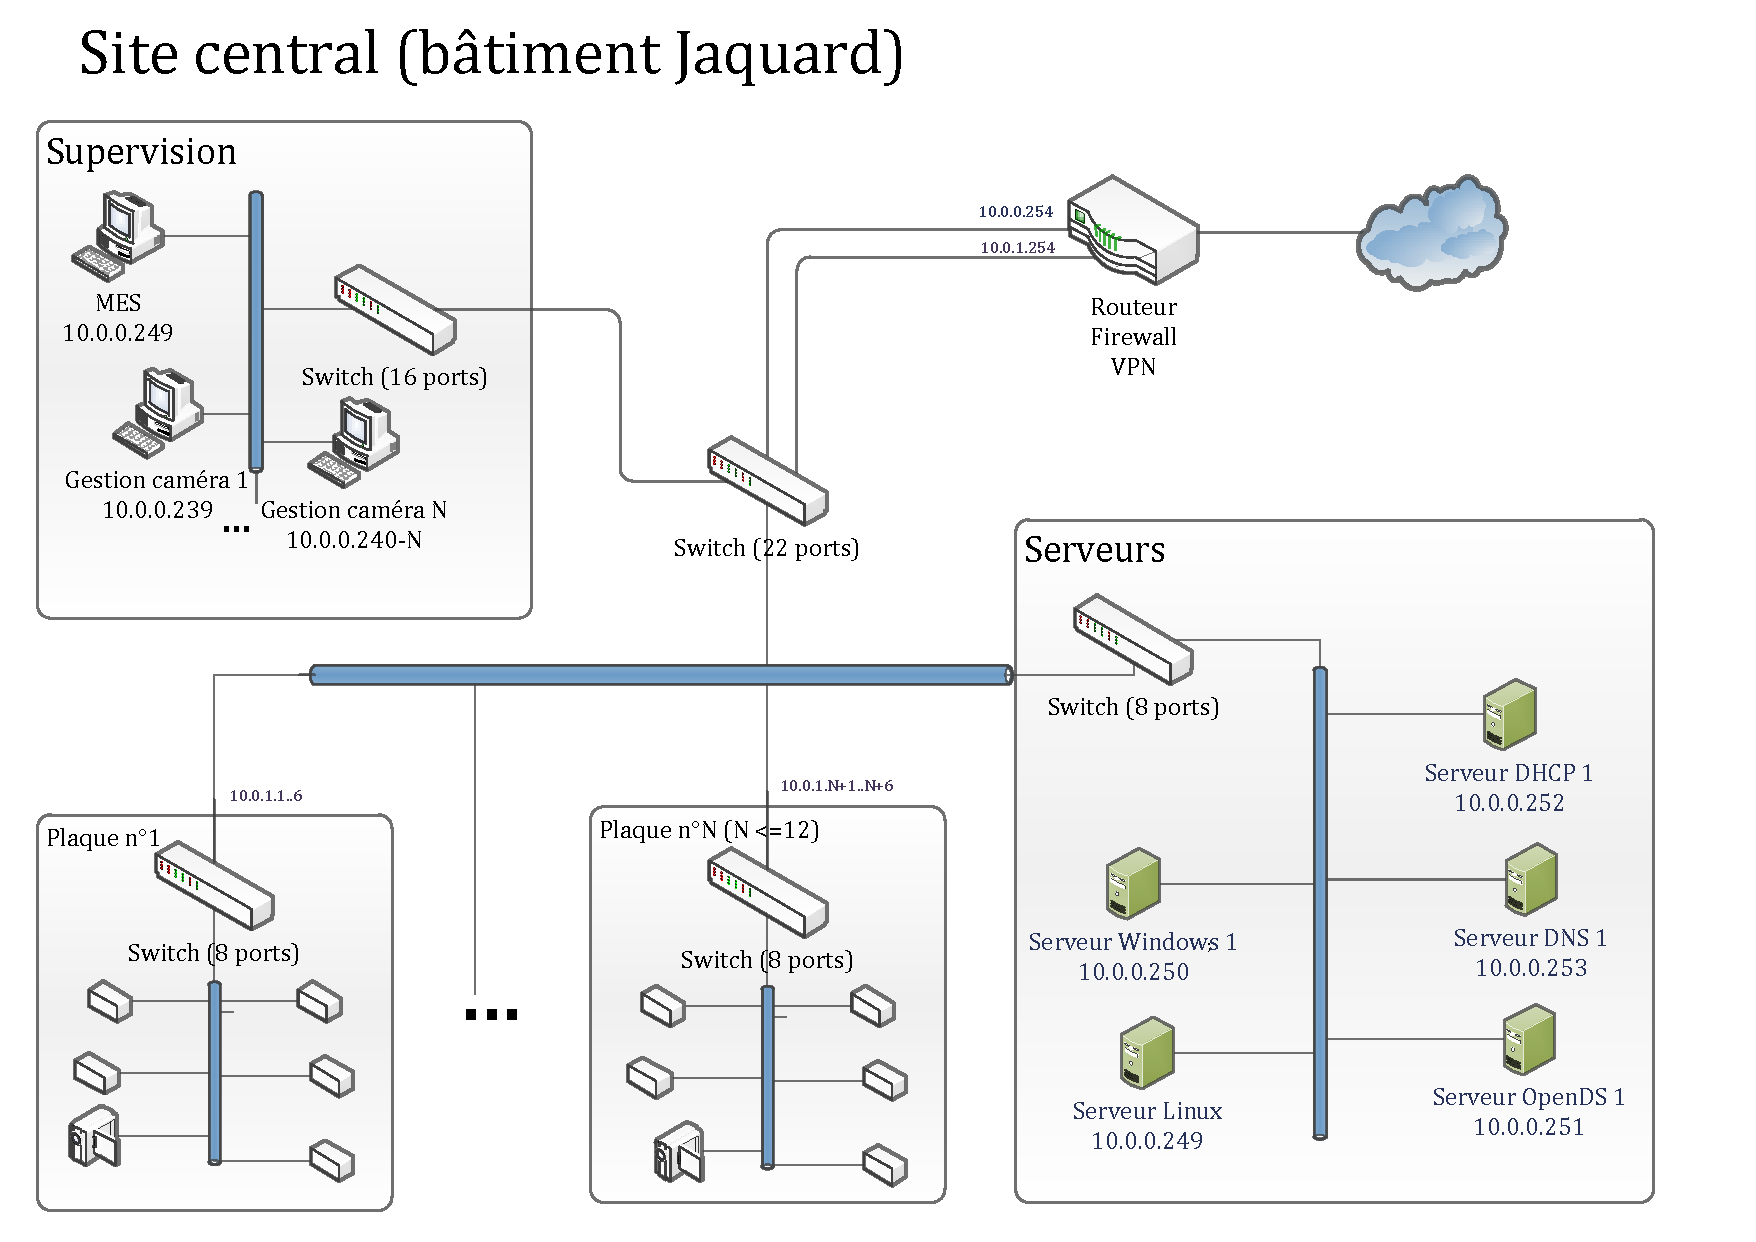
\includegraphics[width=250mm]{\PIXPATH/central}
    \caption{Architecture du site central}
    \label{ac}
\end{sidewaysfigure}
\end{center}

\subsection{Site GE (cf. figure \ref{ag})}

Le {\bf site GE}, situé lui aussi sur le campus de la Doua, bâtiment
        Ferrié, dispose d'un serveur vidéo et de 4 automates programmables.

\begin{center}
\begin{sidewaysfigure}[!h]
    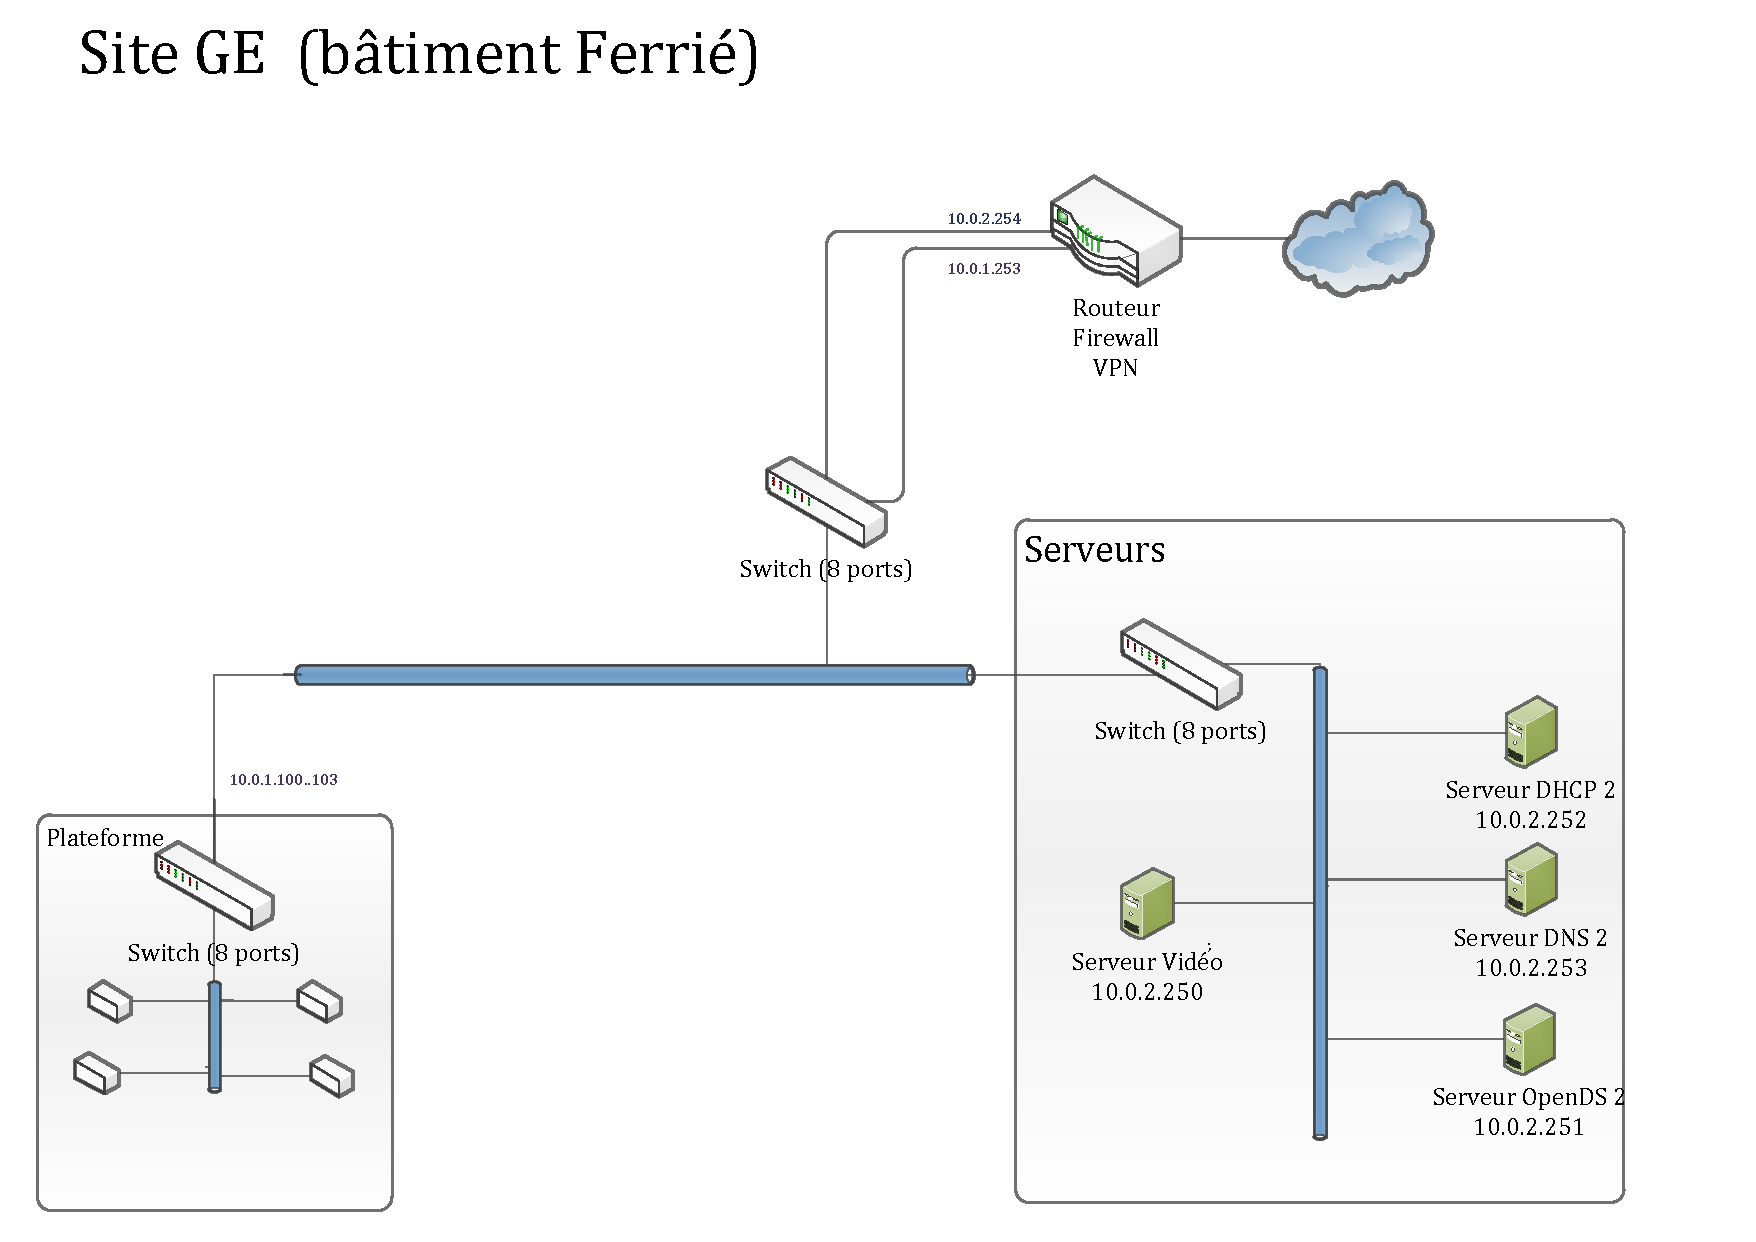
\includegraphics[width=250mm]{\PIXPATH/GE}
    \caption{Architecture du site GE}
    \label{ag}
\end{sidewaysfigure}
\end{center}

\subsection{Site de Roanne (cf. figure \ref{ar})}

Le {\bf site de Roanne}, disposant d'una salle hébergeant des plateformes
        d'automates programmables et d'un serveur Windows.

\begin{center}
\begin{sidewaysfigure}[!h]
    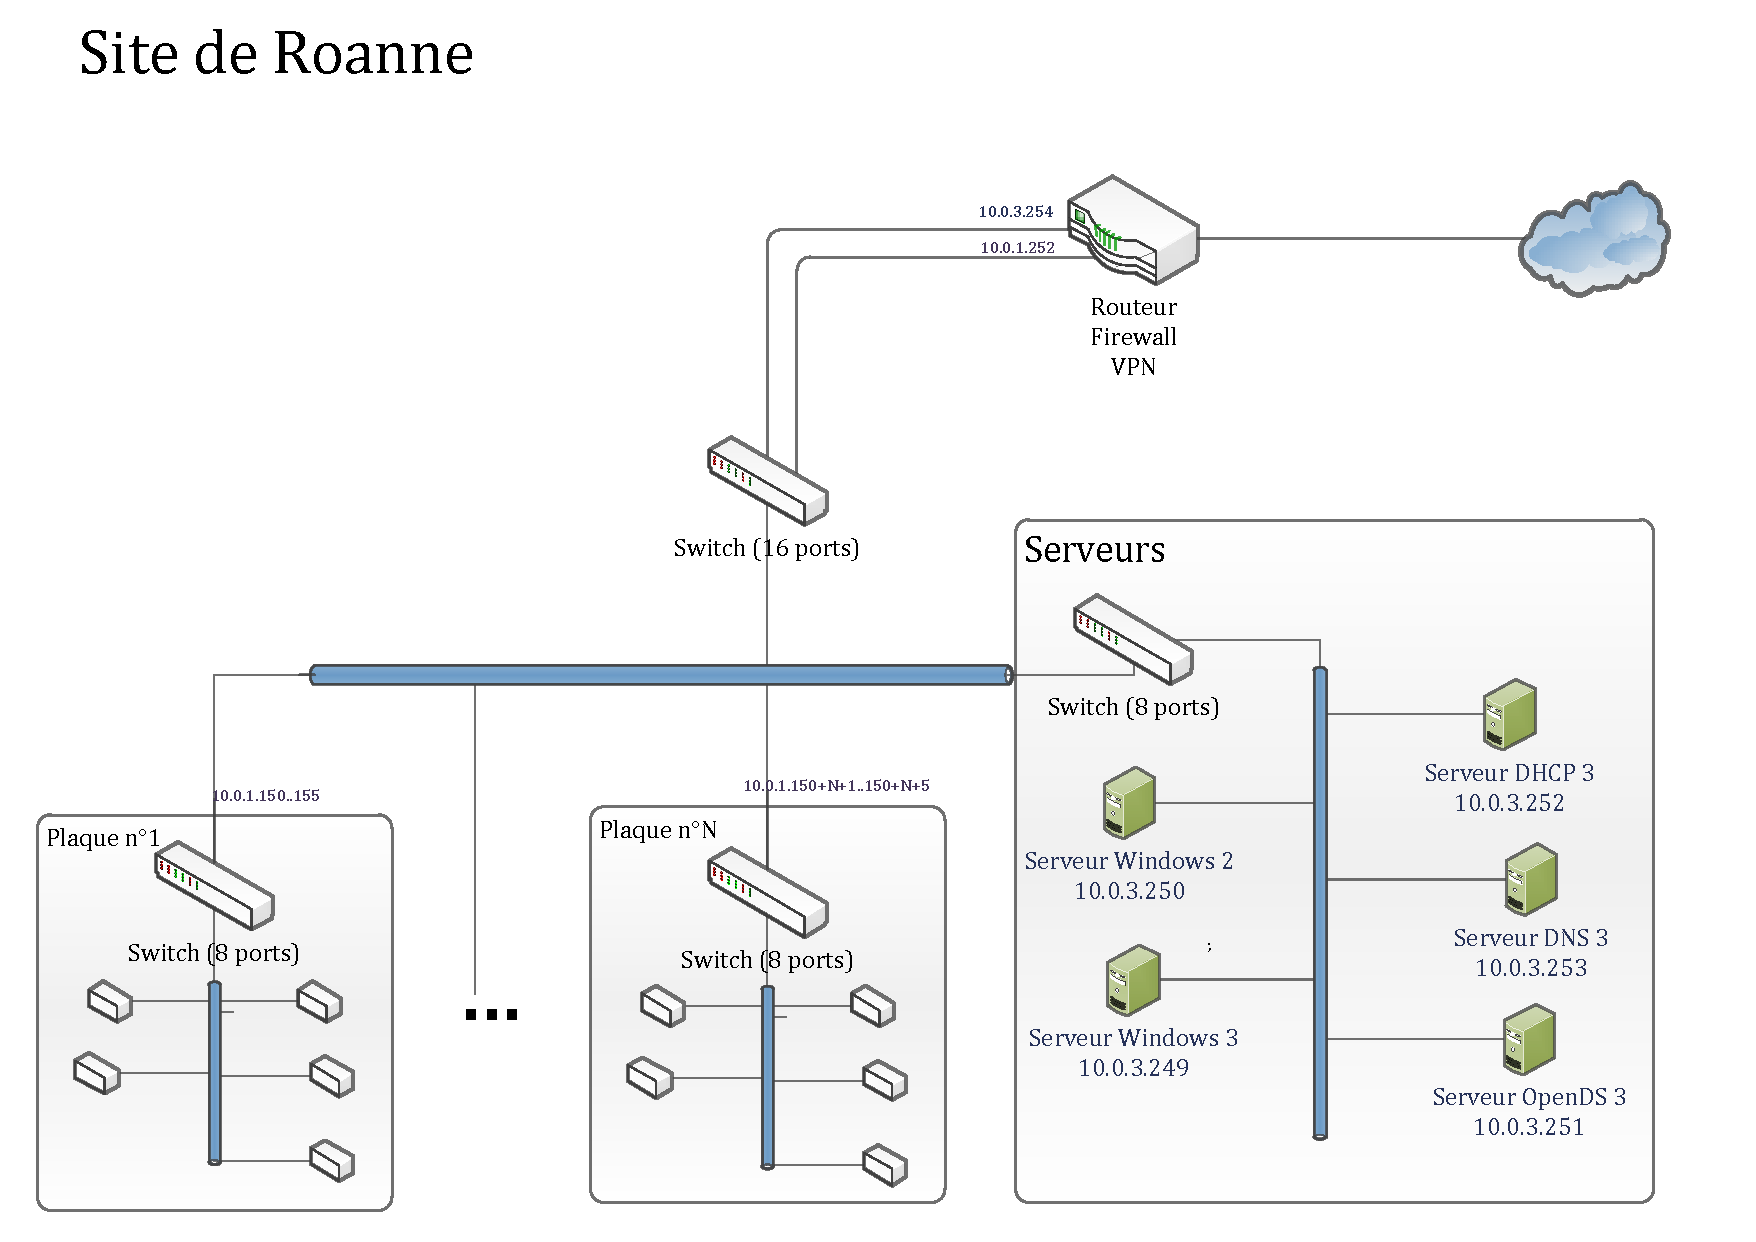
\includegraphics[width=250mm]{\PIXPATH/Roanne}
    \caption{Architecture du site de Roanne}
    \label{ar}
\end{sidewaysfigure}
\end{center}

\FloatBarrier

